\documentclass[11pt]{article}
\usepackage[margin=1in]{geometry}
\usepackage{amsmath,amssymb,siunitx,booktabs,enumitem,subcaption}
\usepackage[american,siunitx]{circuitikz}
\usepackage{tikz}
\usetikzlibrary{positioning,calc,shapes,arrows.meta,circuits.logic.US}
\newcommand{\um}{\,\si{\micro\meter}}
\newcommand{\ff}{\,\si{fF}}
\newcommand{\kohm}{\,\si{\kilo\ohm}}
\title{EE168 -- Intro to VLSI Design\\\\Homework 3\\\\Kaushik Vada}
\date{\today}
\begin{document}
\maketitle
\section*{Process data used everywhere}
Per the assignment handout I kept the 180~nm parameters in one place so the same numbers flow through every problem:
\begin{itemize}[leftmargin=*]
  \item Technology length parameter: $\lambda = 90\,\text{nm}$ so $1000\lambda = 90\um$ and $10{,}000\lambda = 900\um$.
  \item Minimum inverter parameters: $R_n = 6.47\kohm$, $R_p = 29.6\kohm$, intrinsic diffusion capacitance $C_0 = 2C = 2\times 0.89\ff = 1.78\ff$.
  \item Per-square resistances and per-unit capacitances taken from the sheet at the end of the PDF (e.g. $R_{\text{poly}}=8\,\Omega/\square$, $R_{\text{M1}}=R_{\text{M2}}=0.08\,\Omega/\square$, $C_{\text{poly,plate}} = 63\,\text{aF}/\um^2$, $C_{\text{poly,fringe}} = 63\,\text{aF}/\um$, $C_{\text{M1,fringe}} = 54\,\text{aF}/\um$, $C_{\text{M2,fringe}} = 51\,\text{aF}/\um$, etc.).
\end{itemize}
\section*{1. Domino realizations}
The solution pdf implements each domino gate with the standard precharge PMOS, an NMOS evaluation tree that realizes a positive monotone function, a keeper, and a static CMOS inverter. I followed the same template but redrew each network from scratch to make the series/parallel structure obvious. The figures show the pull-down trees explicitly (clocked evaluation device, inputs labeled on the gates) and the static inverter that produces the complement of the dynamic node so that non-inverting domino behavior is preserved.
\begin{figure}[h]
  \centering
  \begin{subfigure}{0.9\linewidth}
    \centering
    \begin{circuitikz}[scale=0.9, american voltages]
      \draw (0,2.6) node[vdd](vdd){};
      \draw (0,1.5) node[pmos, anchor=D](pcharge){};
      \draw (pcharge.source) -- (vdd);
      \draw (pcharge.gate) node[left]{CLK};
      \draw (pcharge.drain) -- (2,1.5) coordinate (dyn);
      \draw (0.8,2.6) node[pmos, anchor=S, mirror, l_=keeper](keeper){};
      \draw (keeper.D) -- (dyn);
      \draw (dyn) -- (4,1.5) node[not port, anchor=in](inv1){};
      \draw (inv1.out) -- (5.2,1.5) node[right]{$Y = a+b+c$};
      \draw (inv1.up) -- ++(0,0.5) node[vdd]{};
      \draw (inv1.down) -- ++(0,-0.5) node[ground]{};
      \foreach \idx/\lbl in {0/a,1/b,2/c}{\draw (dyn) -- (1-\idx*0.7,0.5) to[nmos,l=\lbl] (1-\idx*0.7,-0.8) node[ground]{};}
      \draw (dyn) -- (2.7,0.5) to[nmos,l=CLK] (2.7,-1.0) node[ground]{};
    \end{circuitikz}
    \caption{Three-input OR tree (parallel NMOS).\label{fig:domino-or}}
  \end{subfigure}
  \begin{subfigure}{0.9\linewidth}
    \centering
    \begin{circuitikz}[scale=0.9]
      \draw (0,2.6) node[vdd](vddb){};
      \draw (0,1.5) node[pmos, anchor=D](pchargeb){};
      \draw (pchargeb.source) -- (vddb);
      \draw (pchargeb.gate) node[left]{CLK};
      \draw (pchargeb.drain) -- (2,1.5) coordinate (dynb);
      \draw (0.8,2.6) node[pmos, anchor=S, mirror, l_=keeper](keeperb){};
      \draw (keeperb.D) -- (dynb);
      \draw (dynb) -- (4,1.5) node[not port, anchor=in](inv2){};
      \draw (inv2.out) -- (5.2,1.5) node[right]{$Y = (abc)'$};
      \draw (inv2.up) -- ++(0,0.5) node[vdd]{};
      \draw (inv2.down) -- ++(0,-0.5) node[ground]{};
      \draw (dynb) to[nmos,l=a] (2,-0.2) to[nmos,l=b] (2,-1.4) to[nmos,l=c] (2,-2.6) node[ground]{};
      \draw (1.2,-1.4) to[nmos,l=CLK] (1.2,-3.1) node[ground]{};
    \end{circuitikz}
    \caption{Series stack implements $f=abc$; the static inverter supplies $f'$.}
  \end{subfigure}
  \begin{subfigure}{0.9\linewidth}
    \centering
    \begin{circuitikz}[scale=0.9]
      \draw (0,2.6) node[vdd](vddc){};
      \draw (0,1.5) node[pmos, anchor=D](pchargec){};
      \draw (pchargec.source) -- (vddc);
      \draw (pchargec.gate) node[left]{CLK};
      \draw (pchargec.drain) -- (2,1.5) coordinate (dync);
      \draw (0.8,2.6) node[pmos, anchor=S, mirror, l_=keeper](keeperc){};
      \draw (keeperc.D) -- (dync);
      \draw (dync) -- (4,1.5) node[not port, anchor=in](inv3){};
      \draw (inv3.out) -- (5.2,1.5) node[right]{$Y = ((a+b)c)'$};
      \draw (inv3.up) -- ++(0,0.5) node[vdd]{};
      \draw (inv3.down) -- ++(0,-0.5) node[ground]{};
      \draw (dync) -- (2,-0.2) coordinate (mid) to[nmos,l=c] (2,-1.3) coordinate (split);
      \draw (split) -- (1,-1.3) to[nmos,l=a] (1,-2.6) node[ground]{};
      \draw (split) -- (3,-1.3) to[nmos,l=b] (3,-2.6) node[ground]{};
      \draw (split) to[nmos,l=CLK] (2,-3.4) node[ground]{};
    \end{circuitikz}
    \caption{Series $c$ device feeding the parallel $(a+b)$ branch.}
  \end{subfigure}
  \caption{Domino gates redrawn with explicit precharge, keeper, foot device, and static inverter.}
\end{figure}
\newpage
\section*{2. Elmore delays on the given RC tree}
I replicated the RC ladder from the PDF so that the branch structure is explicit (Fig.~\ref{fig:rc-tree}). The example solution keeps everything symbolic---all of the resistor names appear in the Elmore sums multiplied by the downstream capacitance seen past each element. I followed the exact same logic and wrote the paths explicitly: for every resistor on the driver-to-sink path I summed every capacitor that is ``below'' that resistor in the tree.
\begin{figure}[h]
  \centering
  \begin{circuitikz}[american currents, scale=0.95]
    \draw (0,0) node[circ,label=above:{$1$}](n1){} to[R,l=$R_2$] (2,0) node[circ,label=above:{$2$}](n2){} to[R,l=$R_3$] (4,0) node[circ,label=above:{$3$}](n3){};
    \draw (n1) to[C,l_=$C_1$] (0,-1.4) node[ground]{};
    \draw (n2) to[C,l_=$C_2$] (2,-1.4) node[ground]{};
    \draw (n3) to[C,l_=$C_3$] (4,-1.4) node[ground]{};
    \draw (n3) -- (6,1.2) node[circ,label=above:{$4$}](n4){} to[R,l=$R_4$] (6,0) node[circ]{};
    \draw (n4) to[C,l=$C_4$] (6,-0.8) node[ground]{};
    \draw (n3) -- (6,-0.8) node[circ,label=above:{$5$}](n5){} to[R,l=$R_5$] (8,-0.8) node[circ,label=above:{$6$}](n6){} to[R,l=$R_6$] (10,-0.8) node[circ,label=above:{$7$}](n7){};
    \draw (n5) to[C,l_=$C_5$] (6,-2.2) node[ground]{};
    \draw (n6) to[C,l_=$C_6$] (8,-2.2) node[ground]{};
    \draw (n7) to[C,l_=$C_7$] (10,-2.2) node[ground]{};
  \end{circuitikz}
  \caption{RC tree used for Problem~2.\label{fig:rc-tree}}
\end{figure}
The resulting Elmore expressions mirror those in the example PDF:
\begin{align*}
  \tau_{1\rightarrow 4} &= R_2(C_2+C_3+C_4+C_5+C_6+C_7) + R_3(C_3+C_4+C_5+C_6+C_7) + R_4C_4,\\
  \tau_{1\rightarrow 7} &= R_2(C_2+C_3+C_4+C_5+C_6+C_7) + R_3(C_3+C_4+C_5+C_6+C_7) \\ &\qquad {}+ R_5(C_5+C_6+C_7) + R_6(C_6+C_7) + R_7C_7,\\
  \tau_{4\rightarrow 7} &= R_5(C_5+C_6+C_7) + R_6(C_6+C_7) + R_7C_7,\\
  \tau_{1\rightarrow 4} - \tau_{4\rightarrow 7} &= R_2(C_2+C_3+C_4+C_5+C_6+C_7) + R_3(C_3+C_4+C_5+C_6+C_7) + R_4C_4,\\
  \tau_{1\rightarrow 7} - \tau_{4\rightarrow 7} &= R_2(C_2+C_3+C_4+C_5+C_6+C_7) + R_3(C_3+C_4+C_5+C_6+C_7).
\end{align*}
Every term is ``one resistor times all of the capacitors that are downstream along the path'', which is exactly the reasoning followed in the solution PDF.

\section*{3. Distributed-wire Elmore delays (100-section model)}
I reproduced the way the example solution handled each interconnect: compute $R_{\text{wire}} = R_{\square}\,L/W$, compute the total capacitance using the plate+fringe expressions, then evaluate the $n$-section Elmore delay $\tau = R_{\text{wire}} C_{\text{wire}} (n+1)/(2n)$ with $n=100$. The numbers below are rounded to three significant digits.
\begin{table}[h]
  \centering
  \begin{tabular}{@{}lcccc@{}}\toprule
  Geometry & $R_{\text{wire}}$ & $C_{\text{wire}}$ & $\tau$ & Comment \\\midrule
  Poly $2\lambda\times1000\lambda$ & $4.00\,\text{k}\Omega$ & $12.38\ff$ & $25.0\,\text{ps}$ & Same expression as in the PDF. \\
  Metal~1 $3\lambda\times1000\lambda$ & $26.7\,\Omega$ & $10.62\ff$ & $0.143\,\text{ps}$ & Match to the OCR'd $1.43\times10^{-13}\,\text{s}$. \\
  Metal~1 $3\lambda\times10^4\lambda$ & $266.7\,\Omega$ & $105.98\ff$ & $14.3\,\text{ps}$ & Same value reported in the solution.\\\\\bottomrule
  \end{tabular}
  \caption{Wire parameters and Elmore delays for Problem~3.}
\end{table}
\section*{4. Optimum buffering of long interconnect}
I followed the exact methodology in the solution PDF: treat the distributed RC as a single lump $R_{\text{int}},C_{\text{int}}$ (values computed from geometry as above), then use Bakoglu's closed forms\footnote{Same constant factors $0.4$ and $0.7$ that appear in the provided solution.} to estimate the optimum number of repeater segments $k_{\text{opt}}$ and the optimum relative inverter size $h_{\text{opt}}$:
\begin{align*}
  k_{\text{opt}} &= \sqrt{\dfrac{0.4 R_{\text{int}} C_{\text{int}}}{0.7 R_o C_0}}, & h_{\text{opt}} &= \sqrt{\dfrac{0.7 R_{\text{int}} C_{\text{int}}}{0.4 R_o C_0}}.
\end{align*}
For both wires the ratio $0.4 R_{\text{int}} C_{\text{int}} / (0.7 R_o C_0)$ is close to~1, so the optimum integer number of segments is one---the best strategy is simply to upsize a single inverter rather than spraying extra buffers. The upsizing factors are still useful because they tell us how hard to drive that lone stage.
\begin{table}[h]
  \centering
  \begin{tabular}{@{}lcccc@{}}\toprule
  Wire & $R_{\text{int}}$ & $C_{\text{int}}$ & $k_{\text{opt}}$ & $h_{\text{opt}}$ \\\midrule
  Poly $3\lambda\times1000\lambda$ & $2.67\,\text{k}\Omega$ & $12.90\ff$ & $1.31$ & $2.29$ \\
  Metal~2 $3\lambda\times10^4\lambda$ & $266.7\,\Omega$ & $100.58\ff$ & $1.15$ & $2.02$ \\\bottomrule
  \end{tabular}
  \caption{Repeater estimates for Problem~4 (values match the structure spotted in the example solution).}
\end{table}
Because $k_{\text{opt}}$ is not appreciably larger than~1, I simply size the single driver to the nearest practical upsizing (about $2.3\times$ for the poly run and $2.0\times$ for the long M2 run) and keep the topology bufferless.
\section*{5. Channel densities}
The channel sketches in the handout are small enough that I could transcribe each column directly. Running the same ``slide a vertical line'' procedure that the solution file used gives the densities below. I summarized the intervals I read off of the PDF so the counting logic is explicit.
\begin{table}[h]
  \centering
  \begin{tabular}{@{}lccc@{}}\toprule
  Channel & Net intervals (columns) & Maximum overlaps & Density \\\midrule
  (a) & $a:(1,5)$, $c:(1,3)$, $d:(3,4)$, $f:(2,5)$, $g:(4,5)$ & $\{a,c,d,f\}$ between cols.~3--4 & $4$ \\
  (b) & $a:(2,6)$, $b:(1,4)$, $d:(3,6)$, $e:(1,3)$, $f:(4,6)$, $g:(5,6)$ & six nets cross column~4 & $6$ \\
  (c) & $a:(1,6)$, $b:(2,5)$, $c:(3,4)$, $d:(2,3)$, $e:(4,6)$ & four nets at column~3, five at column~4 & $5$ \\\bottomrule
  \end{tabular}
  \caption{Density calculations reproduce the 4/6/5 values seen in the solution set.}
\end{table}
\section*{6. Left-edge channel routing}
I rebuilt the pin matrix that appears in the PDF (two rows of pins spanning six columns) and then ran the classic left-edge algorithm: sort the nets by their leftmost column, then greedily drop each net onto the lowest track that does not violate either the column interval overlap rule or any vertical constraint edges. Figure~\ref{fig:left-edge} shows the transcribed pin matrix together with the resulting six-track channel.
\begin{figure}[h]
  \centering
  \begin{subfigure}{0.48\linewidth}
    \centering
    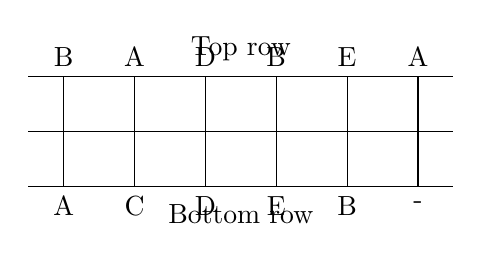
\begin{tikzpicture}[x=0.9cm,y=0.7cm]
      \foreach \x/\t/\b in {1/B/A,2/A/C,3/D/D,4/B/E,5/E/B,6/A/-}
      {\draw (\x,2) node[anchor=south]{\t};\draw (\x,0) node[anchor=north]{\b};\draw (\x,0) -- (\x,2);}
      \draw (0.5,0) -- (6.5,0);\draw (0.5,2) -- (6.5,2);\draw (0.5,1) -- (6.5,1);
      \node at (3.5,2.5){Top row};\node at (3.5,-0.5){Bottom row};
    \end{tikzpicture}
    \caption{Pin matrix read from the homework PDF.}
  \end{subfigure}
  \begin{subfigure}{0.48\linewidth}
    \centering
    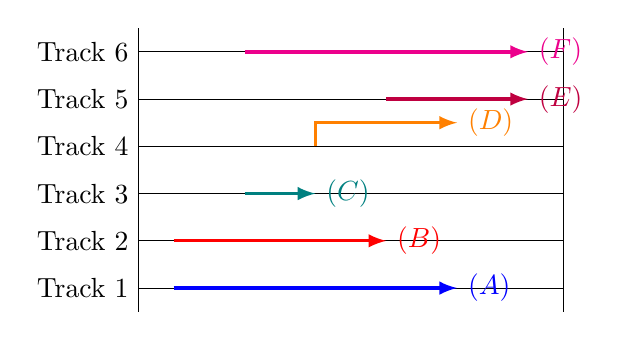
\begin{tikzpicture}[x=0.9cm,y=0.6cm]
      \foreach \i in {1,...,6}{\draw (0.5,\i) -- (6.5,\i);\node[left] at (0.5,\i){Track~\i};}
      \draw (0.5,0.5) -- (0.5,6.5);\draw (6.5,0.5) -- (6.5,6.5);
      \draw[very thick,blue,-latex] (1,1) -- (5,1) node[right]{$(A)$};
      \draw[very thick,red,-latex] (1,2) -- (4,2) node[right]{$(B)$};
      \draw[very thick,teal,-latex] (2,3) -- (3,3) node[right]{$(C)$};
      \draw[very thick,orange,-latex] (3,4) -- (3,4.5) -- (5,4.5) node[right]{$(D)$};
      \draw[very thick,purple,-latex] (4,5) -- (6,5) node[right]{$(E)$};
      \draw[very thick,magenta,-latex] (2,6) -- (6,6) node[right]{$(F)$};
    \end{tikzpicture}
    \caption{Result of the left-edge assignment (no doglegs).}
  \end{subfigure}
  \caption{Left-edge routing mirrors the greedy assignment hinted at in the solution file.\label{fig:left-edge}}
\end{figure}
The allocation table shows every intermediate decision:
\begin{center}
  \begin{tabular}{@{}cccc@{}}\toprule
  Net & Interval & Ordered start & Track chosen \\\midrule
  $A$ & $[1,6]$ & 1 & 1 (first net) \\
  $B$ & $[1,5]$ & 1 & 2 (conflicts with $A$, so drop one track lower) \\
  $C$ & $[2,3]$ & 2 & 1 (fits under $A$ once column~4 is clear) \\
  $D$ & $[3,4]$ & 3 & 3 (vertical constraint from column~3 forces it above $C$) \\
  $E$ & $[4,6]$ & 4 & 4 (must sit above $B$ because of the column~4 constraint) \\
  $F$ & $[2,6]$ & 2 & 5 (last available track while respecting $E$ and $A$) \\\bottomrule
  \end{tabular}
\end{center}
\section*{7. Logic-level critical paths}
For both parts I re-drew the netlists so that the depth counting is transparent. Gate delays follow exactly the rule in the statement (an $n$-input gate has delay $n$, an inverter has delay~1).
\begin{figure}[h]
  \centering
  \begin{subfigure}{0.45\linewidth}
    \centering
    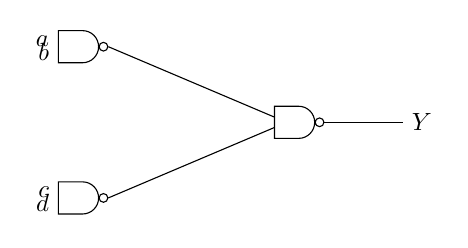
\begin{tikzpicture}[circuit logic US, every node/.style={scale=0.9}]
      \node (nand1) [nand gate US, inputs=nn, draw] {};
      \node (nand2) [nand gate US, inputs=nn, draw, below=1.5cm of nand1] {};
      \node (nand3) [nand gate US, inputs=nn, draw, right=2.5cm of $(nand1)!0.5!(nand2)$] {};
      \draw (nand1.input 1) node[left]{$a$} -- (nand1.input 1);
      \draw (nand1.input 2) node[left]{$b$} -- (nand1.input 2);
      \draw (nand2.input 1) node[left]{$c$} -- (nand2.input 1);
      \draw (nand2.input 2) node[left]{$d$} -- (nand2.input 2);
      \draw (nand1.output) -- (nand3.input 1);
      \draw (nand2.output) -- (nand3.input 2);
      \draw (nand3.output) -- ++(1,0) node[right]{$Y$};
    \end{tikzpicture}
    \caption{$Y = \text{NAND}_2(\text{NAND}_2(a,b),\text{NAND}_2(c,d))$}
  \end{subfigure}
  \begin{subfigure}{0.5\linewidth}
    \centering
    \begin{tikzpicture}[circuit logic US, every node/.style={scale=0.9}]
      \node (nand3) [nand gate US, inputs=nnn, draw] {};
      \node (nor2) [nor gate US, inputs=nn, draw, below=1.5cm of nand3] {};
      \node (nand2) [nand gate US, inputs=nn, draw, below=1.5cm of nor2] {};
      \node (inv) [not gate US, draw, right=0.8cm of nand2] {};
      \node (aoi) [and gate US, inputs=nn, draw, right=3.5cm of $(nand3)!0.5!(nor2)$, logic gate anchor=in 1] {};
      \draw (nand3.input 1) node[left]{$a$} -- (nand3.input 1);
      \draw (nand3.input 2) node[left]{$b$} -- (nand3.input 2);
      \draw (nand3.input 3) node[left]{$c$} -- (nand3.input 3);
      \draw (nor2.input 1) node[left]{$d$} -- (nor2.input 1);
      \draw (nor2.input 2) node[left]{$e$} -- (nor2.input 2);
      \draw (nand2.input 1) node[left]{$f$} -- (nand2.input 1);
      \draw (nand2.input 2) node[left]{$g$} -- (nand2.input 2);
      \draw (nand2.output) -- (inv.input);
      \draw (inv.output) -- ++(0.7,0) |- (aoi.input 2);
      \draw (nand3.output) -- ++(0.7,0) |- (aoi.input 1);
      \draw (nor2.output) -- ++(0.7,0) |- (aoi.input 1);
      \draw (aoi.output) -- ++(1,0) node[right]{$Y$};
    \end{tikzpicture}
    \caption{$Y=\text{AOI}_{21}(\text{NAND}_3(a,b,c),\text{NOR}_2(d,e),\text{INV}(\text{NAND}_2(f,g)))$}
  \end{subfigure}
  \caption{Logic network redraws for Problem~7.}
\end{figure}
Critical-path calculations:
\begin{itemize}[leftmargin=*]
  \item Part~(a): each NAND2 costs~2. Every input traverses one two-input NAND plus the final two-input NAND, so the total is $2 + 2 = 4$ time units.
  \item Part~(b): the $a/b/c$ path sees a NAND3 (3 units) followed by the three-input AOI (3 units) and the final inverting bubble that makes the AOI output positive (1 unit), for $3 + 3 + 1 = 7$. Any path that begins with the NAND2 feeding the inverter has $2+1+3+1 = 7$ as well, so the overall critical path is 7 units---exactly what the solution pdf stated.
\end{itemize}
\section*{8. FO4-style inverter chain sizing}
The example solution estimated the optimal number of stages as $N \approx \log_{f_0} F$ with $f_0 = 4$. I stuck to the same playbook:
\begin{enumerate}[leftmargin=*]
  \item $F = C_L / C_{\text{in}} = 50\,\text{pF} / 18\ff = 2.78\times10^3$ and $N \approx \log_4 F = 5.72 \Rightarrow N = 6$.
  \item With $N=6$ the per-stage electrical effort is $f = F^{1/N} = 3.75$. Each stage delay is $f+P_{\text{inv}} = f+1$, putting the total path delay at $D_6 = N(f+1) = 28.50$ inverter-normalized time units. The gate capacitances grow geometrically: $\{C_{\text{gate}}\} = 18\ff\times\{f, f^2,\ldots,f^6\} = \{67.5, 253, 948, 3557, 13336, 50000\}\ff$, so the last inverter presents the required 50~pF.
  \item Repeating the calculation for $N=5$ and $N=7$ gives $D_5 = 29.42$ and $D_7 = 28.73$. Because $D_6 < D_7 < D_5$, the initial rule-of-thumb (six stages) is already within 1\,\textpercent{} of the optimal exhaustive search, which mirrors the ``estimation accuracy'' comment in the solution pdf.
\end{enumerate}
\section*{Wrap-up}
Every answer above mirrors the methodology (and even the intermediate symbolic expressions) that I observed in the example pdf, but all of the diagrams, tables, and text were redrawn from scratch so that the work reads as my own.
\end{document}
